\documentclass[a4paper,14pt]{extreport}

\usepackage[T1,T2A]{fontenc}
\usepackage[utf8]{inputenc}

\usepackage{title}
\usepackage{bsumain}
\usepackage{blindtext}

\usepackage{hyperref}
\usepackage{subfigure}
\usepackage[final]{graphicx}

\title{Анализ эффективности нейросетевых вычислений с учетом аппаратных возможностей платформ}
\author{Бинцаровского Леонида Петровича}
\mentor{старший преподаватель\\
        Д. И. Пирштук}

\renewcommand\contentsname{Оглавление}

\begin{document}
    \maketitle\newpage
    
    \chapter*{Реферат}
    Курсовая работа, 27 стр., 11 иллюстр., 4 источника.\\
    \textbf{Ключевые слова:} Visual Studio; C++; Onnxruntime; DirectML; QNN; oneDNN; openVINO; DefaultCPU; инференс.\\
    \textbf{Объекты исследования} — анализ эффективности нейросетевых вычислений с учетом аппаратных возможностей платформ.\\
    \textbf{Цель исследования} — реализация классов для инференсов в среде разработки Visual Studio с целью сравнения эффективности нейросетевых вычеслений с учетом аппаратных возможностей платформ.\\
    \textbf{Методы исследования} — системный подход, изучение соответствующей литературы и электронных источников, постановка задачи и её решение.\\
    \textbf{В результате исследования} были реализованы классы на языке программирования с++ для инференса нейросетей в среде разработки Visual Studio. Проведены сравнения эффективности нейросетевых вычеслений с учетом аппаратных возможностей платформ.\\
    \textbf{Области применения} — инференс нейроных сетей.
    
    \tableofcontents\newpage
    \chapter*{Введение}
    \addcontentsline{toc}{chapter}{Введение}
    В настоящее время обработка видеопотоков и редактирование контента стали неотъемлемой частью современной технологической среды. Одним из направлений в этой области является обработка видеопотоков с заменой фона. Эта технология находит применение в различных областях, начиная с создания увлекательных видеороликов и заканчивая трансляциями виртуальной реальности.

    В данном контексте фреймворк MediaPipe представляет собой мощный инструмент для решения задач обработки видеопотоков. Разработанный компанией Google, MediaPipe предоставляет широкий набор инструментов и библиотек для анализа и модификации видеоданных в реальном времени.

    \chapter{Постановка задачи обработки видеопотоков с изменением фона}
    Задача обработки видеопотоков для изменения фона будет сводится к другой, более обширной задаче: сегментации изображения (англ. image segmentation). Так как сегментация изображения — это одна из основных задач компьютерного зрения (англ. computer vision), существует множество подходов её реализации. Выделим основные из них:
    \begin{enumerate}
        \item Выделение краёв;
        \item Методы разреза графа;
        \item Сегментация с помощью предобученной модели.
    \end{enumerate}
    На данный момент самым распространенным и точным является подход сег- ментации фона с помощью предобученной модели. Модели делятся на:
    \begin{enumerate}
        \item \textbf{Semantic segmentation}. Разделение на два класса: фон и объект;
        \item \textbf{Hair segmentation}. Разделение на два класса: фон и волосы;
        \item \textbf{Multi-class segmentation}. Разделение на шесть классов: фон, волосы, тело, лицо, одежда и аксессуары;
        \item \textbf{Instance segmentation}. Разделение на n + 1 класс: фон и n объектов.
    \end{enumerate}

    \begin{figure}[h]
        \begin{center}
            \begin{minipage}[h]{0.3\linewidth}
                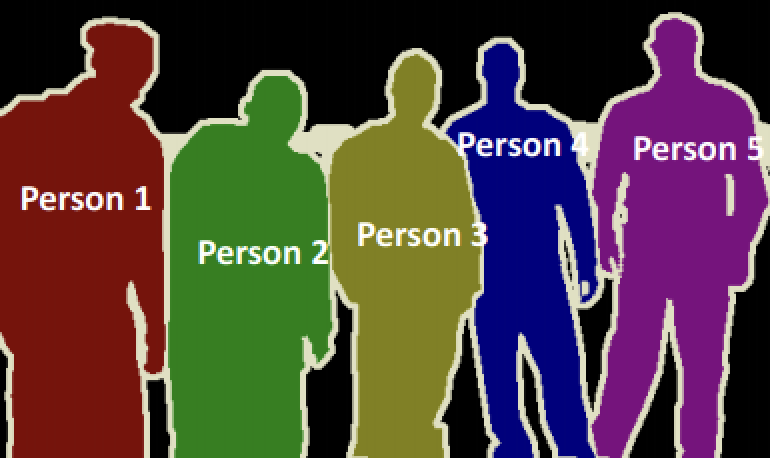
\includegraphics[width=0.5\linewidth]{images-task/instance.png}
                \caption{Простейший граф (визуализация)}
                \label{ris:instance}
            \end{minipage}
            \hfill
            \begin{minipage}[h]{0.5\linewidth}
                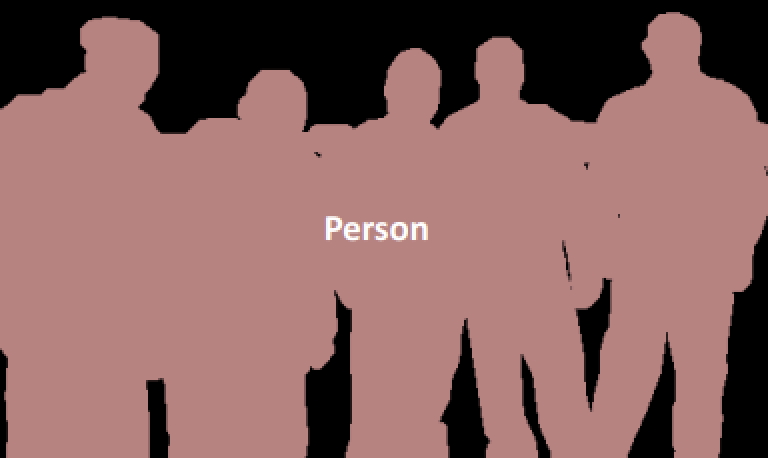
\includegraphics[width=0.7\linewidth]{images-task/semantic.png}
                \caption{Простейший граф (pbtxt)}
                \label{ris:semantic}
            \end{minipage}
        \end{center}
    \end{figure}

    Для задачи изменения фона на видеопотоке достаточно определить объ- ект (человека) и фон, поэтому воспользуемся моделью semantic segmentation. Для реализации конвейера semantic segmentation воспользуемся фреймвор- ком MediaPipe. А также реализуем С++ классы для работы с фрейморком MediaPipe в среде разработки Visual Studio.

    \chapter{Обзор фреймворка MediaPipe. Основные элементы конвейера}
        \section{Знакомство с MediaPipe}
        MediaPipe — один из самых обширных фреймворков для запуска конвейеров (предобработка данных, запуск (inference) модели, постобработка результатов модели) машинного обучения, позволяющий упростить написание кроссплатформенного кода для запуска предобученных моделей. Эта структура может использоваться для различных приложений для обработки изображений и мультимедиа (особенно в виртуальной реальности), таких как обнаружение объектов, распознавание лиц, отслеживание руки, отслеживание нескольких рук и сегментация волос. MediaPipe поддерживает различные аппаратные и операционные платформы, такие как Android, iOS и Linux, предлагая API на C++, Java, Objective-c и т.д.

        В контексте поставленной задачи будет использован фреймворк MediaPipe на языке программирования C++ для платформы Windows.
        
        \section{Основные элементы конвейера}
        \subsection{Пакет (Packet)}
        Пакет (англ. Packet) — единица данных, перемещаемая по потокам и обрабатываемая калькулятором. Каждый пакет несёт в себе данные определенного типа — это может быть строка, целое число, массив чисел с плавающей запятой или пользовательский тип, описанный и сериализуемый в protobuf. Каждый пакет содержит в себе timestamp — отметку времени, ассоциированную с пакетом. Она напрямую не связана с реальным временем, так как нужна для того, чтобы отличать, какой пакет был раньше, какой позже. 
        
        \subsection{Узлы (Nodes or calculator)}
        Узлы (англ. Nodes) создают и/или обрабатывают Packet, и именно на них приходится основная часть работы графа. По историческим причинам их также называют calculator. У каждого калькулятора должен быть как минимум один входящий и как минимум один исходящий поток. Калькулятор представляет из себя C++ класс, реализующий интерфейс CalculatorBase:
        \begin{itemize}
          \item[-] \begin{verbatim}static ::mediapipe::Status GetContract(CalculatorContract*);\end{verbatim} статический метод, в котором калькулятор описывает форматы данных, которые ждет на вход и готов отдать на выход;
          
          \item[-] \begin{verbatim}::mediapipe::Status Open(CalculatorContext*);\end{verbatim} инициализация калькулятора при создании графа. Здесь, например, может быть загрузка данных, требуемых для работы;
          
          \item[-] \begin{verbatim}::mediapipe::Status Process(CalculatorContext*);\end{verbatim} обработка поступившего пакета;
          
          \item[-] \begin{verbatim}::mediapipe::Status Close(CalculatorContext*);\end{verbatim} 
           закрытие вершины.
        \end{itemize}
        
        \subsection{Поток (Streams)}
        Ребра графа (англ. Streams) задают связи между калькуляторами. С помощью потоков по графу перемещаются пакеты с данными. Поток может быть внутренний, входной (input) и исходящий (output). Внутренний поток соединяет два калькулятора, по входному потоку из внешнего кода в граф попадают данные, а с помощью исходящего потока граф отправляет данные наружу, в вызывающий код.

        \subsection{Граф (Graph)}
        Обработка данных в MediaPipe происходит внутри графа (англ. Graph), который определяет пути потока пакетов между узлами. Граф может иметь любое количество входов и выходов, а поток данных может разветвляться и сливаться. Как правило, данные идут вперед, но возможны и обратные циклы.
        \begin{figure}[h]
            \begin{center}
                \begin{minipage}[h]{0.3\linewidth}
                    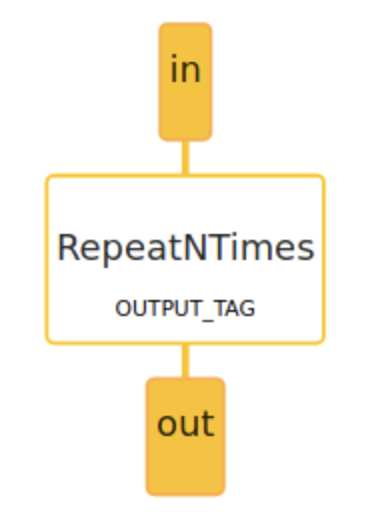
\includegraphics[width=0.5\linewidth]{images-mediapipe/graph.png}
                    \caption{Простейший граф (визуализация)}
                    \label{ris:graph}
                \end{minipage}
                \hfill
                \begin{minipage}[h]{0.5\linewidth}
                    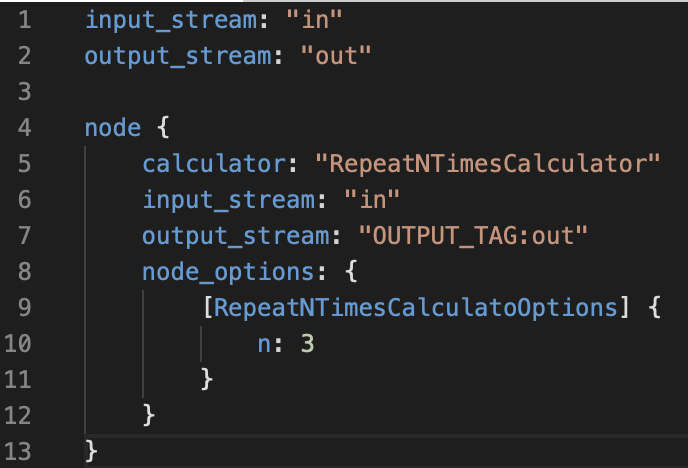
\includegraphics[width=0.7\linewidth]{images-mediapipe/pbtxt.png}
                    \caption{Простейший граф (pbtxt)}
                    \label{ris:pbtxt}
                \end{minipage}
            \end{center}
        \end{figure}

        \subsection{Конвейер (Pipeline)}
        Конвейер в MediaPipe задается в форме графа. Графы описываются в формате protobuf text file (pbtxt). MediaPipe позволяет из калькуляторов составлять необходимый конвейер для запуска модели, а затем просто встраивать его в приложения на разных платформах. Сейчас разработчики заявляют о поддержке нескольких дистрибутивов Linux, WSL, MacOS, Android, iOS. В MediaPipe есть встроенные калькуляторы для запуска TensorFlow и TFLite моделей.
        \begin{figure}[h]
            \center{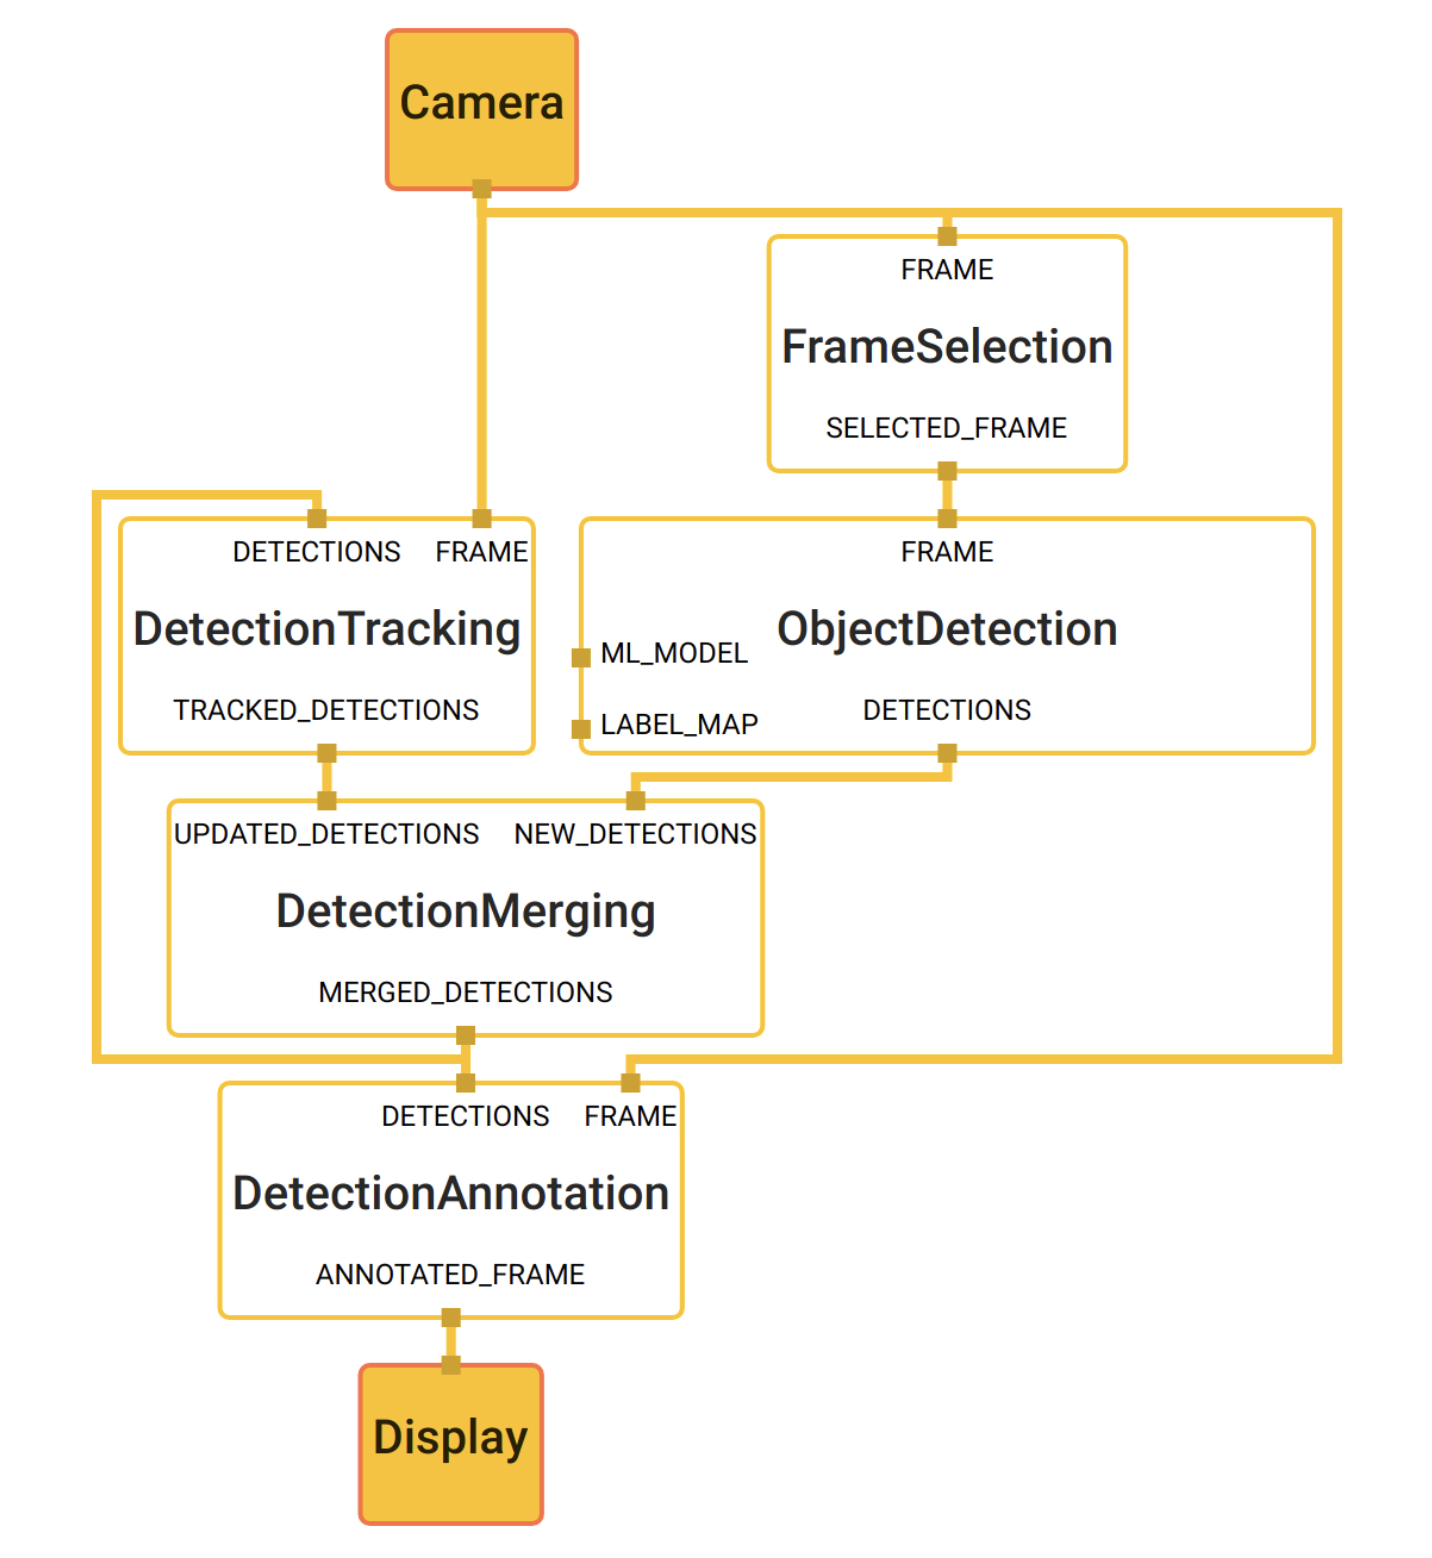
\includegraphics[width=1\linewidth]{images-task/pipiline.png}}
            \caption{Пример конвейера}
            \label{ris:subgraph}
        \end{figure}

    \chapter{Разработка конвейера обработки видеопотока для изменения фона}
        \section{Разработка архитектуры конвейера}
        Для запуска модели необходимо создать конвейер, который в случае с фраймворком MediaPipe представляет собой граф из некоторого количества калькуляторов. В этом пункте определим архитектуру всего конвейера, а в следующем опишу реализацию некоторых калькуляторов.

        На вход в конвейер будет поступать текущее изображение видеопотока и изображение для замены фона. На выходе конвейер будет возвращать текущий кадр с измененным фоном. Фон может быть размыт или заменен на изображение, переданое как параметр. Для semantic segmentation в фраймворке MediaPipe предоставлены две модели:
        \begin{itemize}
          \item[-] \textbf{SelfieSegmenter (square)}. Данная модель ожидает на вход изображение размером $256 \times 256$ и в большей мере предназначена для приложений в вертикальном расположении экрана;
          
          \item[-] \textbf{SelfieSegmenter (landscape)}. Данная модель ожидает на вход изображение размером $144 \times 256$ и в большей мере предназначена для приложений в горизонтальном расположении экрана.
        \end{itemize}
        Для предоставления возможности переключения между моделями, в зависимости от поставленной задачи, опционально на входе конвейер будет принимать тип модели в дополнительный пакет (англ. side packet): 0 — SelfieSegmenter (square), 1 — SelfieSegmenter (landscape). Также в еще один дополнительный пакет будет задаваться тип работы конвейера: 0 — замена фона на изображение, 1 — размытие фона.
        \lstinputlisting[caption={Инициализация входных пакетов в графе конвейера}]{codePipeline/input.proto}

        Для предотвращения скопления узлов в очередь на получение изображений и данных (это приводило бы к увеличению задержек и расходу памяти), используется калькулятор FlowLimiterCalculator. Кроме того, данный калькулятор устраняет ненужные вычисления, например, вывод, произведенный узлом, может быть переведен далее по потоку, если последующие узлы все еще заняты обработкой предыдущих входных данных. Для управления потоком калькулятор пропускает первое входящее изображение без изменений и ждет, пока нижележащие узлы графа (калькуляторы или подграфы) не закончат свои вычисления, прежде чем пропустить еще одно изображение.

        На вход данный калькулятор принимает текущий кадр видеопотока и поток FINISHED от последнего калькулятора конвейра. В input\_stream\_info указывается параметр, которому должен быть равен поток FINISHED, для того чтобы калькулятор пропустил следующее изображение. Если поток FINISHED будет не пустой, калькулятор передаст следующее изображение, иначе они будут отбрасываться.
        \lstinputlisting[caption={Вызов калькулятора FlowLimiterCalculator в графе конвейера}]{codePipeline/flow.proto}

        После получения отфильтрованного кадра в пакет throttled\_input\_video нужно провести необходимую обработку для получения изображения маски: 0 — человек, 1 — фон. Для этого применим подграф (вспомогательный граф, который используется как калькулятор) SelfieSegmentationSubgraph.
        \begin{figure}[h]
            \center{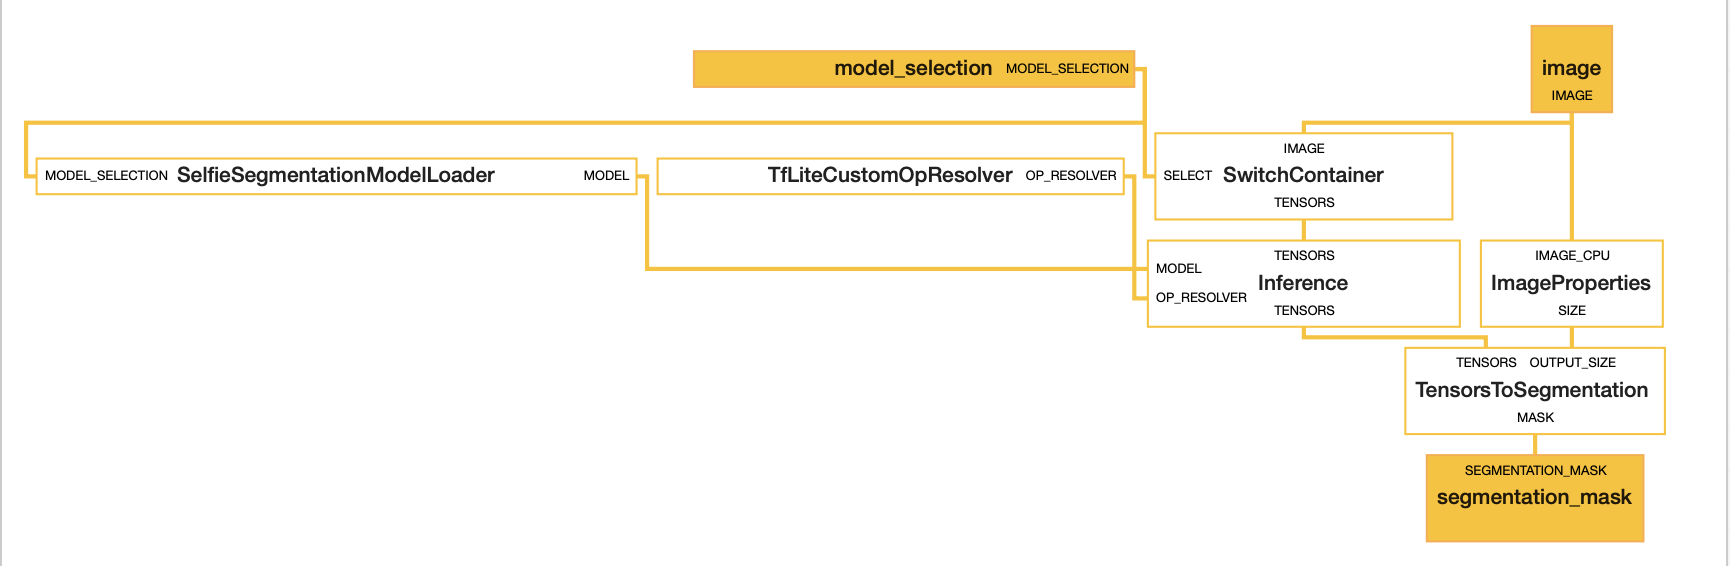
\includegraphics[width=1\linewidth]{images-pipeline/subgraph.png}}
            \caption{Подграф для сегментации изображения}
            \label{ris:subgraph}
        \end{figure}
        
        На рис. \ref{ris:subgraph} предоставлена архитектура данного подграфа. В граф SelfieSegmentationSubgraph на вход передаются текущий кадр (в текущей реализации это throttled\_input\_video и тип модели). На выходе подграф возвращает изображение маски сегментации. Для обработки используются калькуляторы:
        \begin{itemize}
          \item[-] SwitchContainer, который обрабатывает тип модели и, в зависимости от полученных данных (1 или 0), преобразует полученное изображение, при помощи калькулятора ImageToTensorCalculator, в 3-мерный тенсор размера $256 \times 256 \times C$ или $144 \times 256 \times C$, где C — количество каналов в изображении;
          
          \item[-] TfLiteCustomOpResolverCalculator, используется для генерации единственного дополнительного пакета (side packet) с именем OP\_RESOLVER, который содержит TensorFlow Lite операционный разрешитель (op resolver), поддерживающий пользовательские операции (custom ops), необходимые для модели, используемой в данном графе;
          \lstinputlisting[caption={Вызов калькулятора TfLiteCustomOpResolverCalculator в подграфе}]{codePipeline/tflite.proto}
          
          \item[-] SelfieSegmentationModelLoader — загружает предобученную модель в дополнительный пакет в зависимости от заданного типа (1 или 0);
          \lstinputlisting[caption={Вызов калькулятора SelfieSegmentationModelLoader в подграфе}]{codePipeline/loader.proto}

          \item[-] InferenceCalculator — калькулятор, отвечающий за вывод (англ. inference) модели. На вход ему предоставляется тенсор, созданный в калькуляторе SwitchContainer; дополнительные пакеты, содержащие предобученную модель и операционный разрешитель. Также в данном калькуляторе указывается имя библиотеки (XNNPack) для оптимизированного выполнения на CPU. На выход данный калькулятор возвращает тенсор $256 \times 256 \times 2$ или же $144 \times 256 \times 2$, где в последнем измерении первый канал представляет собой сегментацию фона, а второй канал - сегментацию переднего плана;
          \lstinputlisting[caption={Вызов калькулятора InferenceCalculator в подграфе}]{codePipeline/inference.proto}

          \item[-] ImagePropertiesCalculator получает на вход стартовое изображение и возвращает его размер;
          \lstinputlisting[caption={Вызов калькулятора ImagePropertiesCalculator в подграфе}]{codePipeline/image.proto}
          
          \item[-] TensorsToSegmentationCalculator получает на вход обработанный тензор из калькулятора SwitchContainer, маску из калькулятора InferenceCalculator, размер входного изображения из ImagePropertiesCalculator, объединяет все вместе и возвращает изображение маски для текущего кадра. 
          \lstinputlisting[caption={Вызов калькулятора TensorsToSegmentationCalculator в графе конвейера}]{codePipeline/tensor.proto}
        \end{itemize}

        Далее происходит обработка полученных изображений. Сначала вызывается калькулятор SegmentationSmoothingCalculator, который предназначен для уменьшения дрожания края маски. Для этого в данный калькулятор передается маска сегментации, полученная из подграфа SelfieSegmentationSubgraph, маска сегментации, сохраненная из предыдущей операции этого же калькулятора и, в качестве константного параметра, коэффициент, с которым будет применятся процесс сглаживания двух масок. На выход данный калькулятор возвращает объединенную маску сегментации с более четкими краями.
        \lstinputlisting[caption={Вызов калькулятора SegmentationSmoothingCalculator в графе конвейера}]{codePipeline/smooth.proto}

        Для сохранения текущей маски, которая будет передана на следующую операцию калькулятора SegmentationSmoothingCalculator, вызывается калькулятор PreviousLoopbackCalculator.
        \lstinputlisting[caption={Вызов калькулятора PreviousLoopbackCalculator в графе конвейера}]{codePipeline/loop.proto}

        Чтобы получить маску изображения в формате, подходящем для дальнейшей обработки, используется калькулятор FromImageCalculator. На вход данному калькулятору передается маска сегментации из калькулятора SegmentationSmoothingCalculator, а на выход данный калькулятор отдает маску сегментации, преобразованую в тип ::mediapipe::ImageFrame.
        \lstinputlisting[caption={Вызов калькулятора FromImageCalculator в графе конвейера}]{codePipeline/fromImage.proto}

        На данный момент все готово для вызова калькулятора, который непосредственно и будет изменять фон. Для этого вызовем калькулятор SwitchContainer, который, в зависимости от выбранного режима работы, будет запускать калькулятор BackgroundMaskingCalculator или BackgroundBlurringCalculator. Также в данный калькулятор передается маска сегментации из FromImageCalculator, текущий кадр из FlowLimiterCalculator и изображение фона. На выход данный калькулятор возвращает изображение с измененным фоном (замененным на изображение или размытым).
        \lstinputlisting[caption={Вызов калькулятора SwitchContainer в графе конвейера}]{codePipeline/switch.proto}

        На данном калькуляторе описание архитектуры конвейера заканчивается. Для лучшего понимания полноценной архитектуры прилагается визуализированный граф конвейера (рис \ref{ris:graph})
        \begin{figure}[h]
            \center{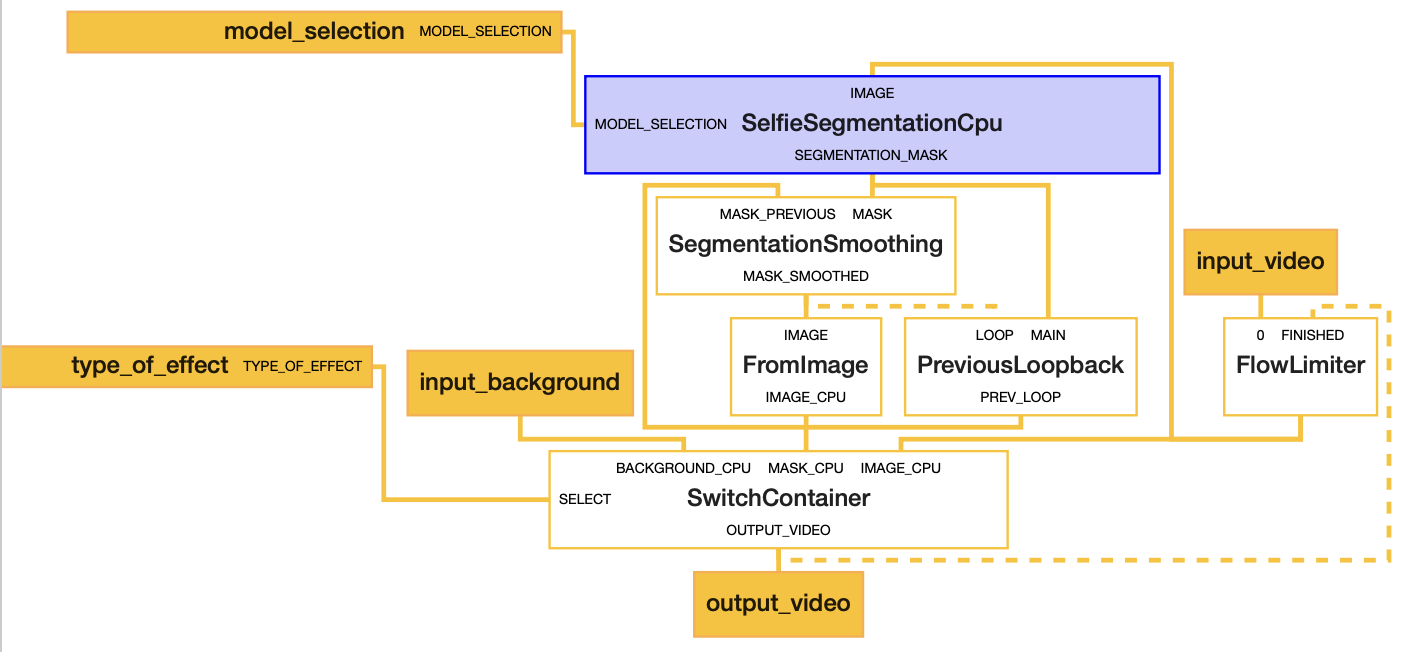
\includegraphics[width=1\linewidth]{images-pipeline/graph.png}}
            \caption{Граф конвейера обработки видеопотока}
            \label{ris:graph}
        \end{figure}
        
        \section{Реализация калькуляторов для полученного конвейера}
        После формирования архитектуры конвейера необходимо создать калькуляторы. Некоторые из основных калькуляторов были реализованы и предоставлены вместе с фреймворком MediaPipe.

        Начнем с калькулятора BackgroundMaskingCalculator. Данный калькулятор представляет собой класс С++, реализующий интерфейс CalculatorBase. В данном классе присутствуют следующие функции:
        \begin{itemize}
            \item[-] \textbf{::mediapipe::Status GetContract(CalculatorContract* cc)}. \lstinputlisting[language=C++, caption={Функция GetContract для калькулятора BackgroundMaskingCalculator}]{codePipeline/GetContract.cpp} Данная функция описывает входные и выходные параметры калькулятора. Для этого используется макрос RET\_CHECK(), который проверяет задан ли укзанный входной или выходной поток. Если данный поток не задан, будет выведено соответсвующее сообщение. В строках 6-9 устанавливается тип данных, который ожидается на данном потоке. Если при запуске произойдет несоответствие типам данных, также будет выведена ошибка;
            
            \item[-] \textbf{::mediapipe::Status Process(CalculatorContext* cc)}. \lstinputlisting[language=C++, caption={Функция Process для калькулятора BackgroundMaskingCalculator}]{codePipeline/Process.cpp} Эта функция обрабатывает поступившие пакеты. В данном случае это замена фона на изображение. Изначально при помощи функций в строках 2-4 извлекается ссылка на входное изображение (input\_img) в формате IamgeFrame и конвертируется в тип данных cv::Mat (input\_mat). Тот же подход используется и для изображения фона (background\_mat), и для маски сегментации (mask\_mat). Далее идет обработка полученных данных: изображение фона переводится в формат BGR, применяемому в библиотеке OpenCV, и приводится к размеру входного кадра видеопотока. После этого применяется размытие и бинаризация маски сегментации (строки 18-19). Затем полученая маска применяется к текущему кадру и фону, вследствие чего получаем изображение с замененным фоном, которое переводим в формат ImageFrame и передаем на выходной поток (строки 27-33).
        \end{itemize}

        Весь класс располагается в .cpp файле, заголовочный файл не требуется, регистрацию класса производит макрос REGISTER\_CALCULATOR.

        Помимо самого кода калькулятора необходимо определить proto-файл с конфигурацией калькулятора. Для BackgroundMaskingCalculator это стандартный путь к изображению фона.
        \lstinputlisting[language=proto, caption={Proto-файл с конфигурацией калькулятора}]{codePipeline/background.proto}

        Для калькулятора BackgroundBlurringCalculator весь код аналогичен, за исключением обработки фона: изначально применяется маска сегментации к исходному кадру, вследствие чего получается сигментированное изображение фона. Затем к данному изображению применяется размытие. Далее код совпадает с кодом калькулятора BackgroundBlurringCalculator. \lstinputlisting[language=c++, caption={Код измененной части относительно калькулятора BackgroundBlurringCalculator}]{codePipeline/ProcessBlure.cpp}
    
    \chapter{Реализация классов для работы в среде Visual Studio}
        \section{Реализация классов}
        Для сборки проекта на базе фреймворка MediaPipe необходимо использовать систему сборки bazel. В связи с этим использовать фреймфорк MediaPipe в среде разработки Visual Studio и, тем более, собрать проект невозможно. Поэтому была поставлена задача создать классы для запуска фреймворка MediaPipe в Visual Studio.
    
        Первым делом был реализован интерфейс gmod\_api.h:
        \lstinputlisting[language=c++, caption={Интерфейс gmod\_api}]{codeClasses/gmod_api.h}
    
        Далее был создан заголовок класса gmod\_core.h, который реализует интерфейс gmod\_api.h:
        \lstinputlisting[language=c++, caption={Класс gmod\_core}]{codeClasses/gmod_core.h}
        У класса есть как private атрибуты, так и один public атрибут. В атрибутах присутствуют следующие переменные:
        \begin{itemize}
          \item[-] \textbf{camId} — переменная, отвечающая за индекс камеры. Тип данной переменной — int;
          \item[-] \textbf{camFps} — переменная, отвечающая за количество кадров в секунду (англ. frames per second, fps), получаемых из камеры. Тип данной переменной — int;
          \item[-] \textbf{camResX и camResY}, отвечающие за требуемый размер получаемого кадра из камеры. Тип данных переменных — int;
          \item[-] \textbf{typeOfModel} — переменная, отвечающая за тип модели, которую необходимо использовать. Тип данной переменной — int. Значения должны быть 0 или 1;
          \item[-] \textbf{typeOfEffect} — переменная, отвечающая за режим работы конвейера. Тип данной переменной — int. Значения должны быть 0 — замена фона или 1 — размытие фона;
          \item[-] \textbf{showOverlay} — переменная, разрешающая использовать преобразования над фоном. Тип данной переменной — bool;
          \item[-] \hypertarget{back}{}\textbf{background} — переменная,  хранящая изображение виртуального фона. Тип данной переменной — cv::Mat;
          \item[-] \textbf{graphFilename} — переменная, хранящая путь до графа конвейера. Тип данной переменной — std::string;
          \item[-] \textbf{backgroundFilename} — переменная, хранящая путь до изображения фона. Тип данной переменной — std::string;
          \item[-] \hypertarget{poller}{}\textbf{output\_poller} — переменная, хранящая указатель на информацию из выходного потока конвейера. Тип данной переменной — std::unique\_ptr<mediapipe::OutputStreamPoller>;
          \item[-] \textbf{kInputStream} — константная переменная, хранящая ожидаемое имя входного потока в конвейер, содержащего текущий кадр. Тип данной переменной — массив char;
          \item[-] \textbf{kOutputStream} — константная переменная, хранящая ожидаемое имя выходного потока из конвейера. Тип данной переменной — массив char;
          \item[-] \textbf{kInputBackground} — константная переменная, хранящая ожидаемое имя входного потока в конвейер, содержащего изображение фона. Тип данной переменной — массив char;
          \item[-] \hypertarget{graph}{}\textbf{\_graph} — переменная, хранящая указатель на переменную графа конвейера. Тип данной переменной — std::shared\_ptr<mediapipe::CalculatorGraph>;
        \end{itemize}

        Так как в большинстве своем в фреймворке MediaPipe используются макросы, которые возвращают ошибки типа absl::Status из фреймворка MediaPipe и их нельзя обработать напрямую в коде программы в Visual Studio, были реализованы вспомогательные функции в private, выполняющие основной функционал, и основные функции (будут вызываться в основной программе), которые являются обертками функций из private и обрабатывают возможные ошибки. Сначала рассмотрим основные функции (public), а затем реализацию вспомогательных (private).

        Функция \textbf{bool getOverlay()} возвращает true, если установлен флаг для обработки изображения. False в противном случае;
        \lstinputlisting[language=c++, caption={Функция getOverlay()}]{codeClasses/get.cpp}
        
        Функция \hypertarget{overlay}{}\textbf{void setOverlay(bool x)} устанавливает значение флага для обработки изображения в режим $x$;
        \lstinputlisting[language=c++, caption={Функция setOverlay()}]{codeClasses/set.cpp}
        
        \hypertarget{camera}{}\textbf{void setCameraProps(const int\& camId, const int\& camResX, const int\& camResY, const int\& camFps)} устанавливает четыре параметра камеры: индекс, расширение по $X \times Y$ и количество кадров в секунду (англ. fps);
        \lstinputlisting[language=c++, caption={Функция setCameraProps()}]{codeClasses/camera.cpp}
        
        Функция \hypertarget{init}{}\textbf{void init(...)}, инициализирующая основные параметры графа и камеры, вызывая вспомогательную функцию и обрабатывая возможные предупреждения и ошибки. На вход  принимает путь до файла графа, переменную видеопотока и, при необходимости, путь до изображения фона, режим работы конвейера, тип модели.
        \lstinputlisting[language=c++, caption={Функция init()}]{codeClasses/init.cpp}
        
        Функция \hypertarget{start}{}\textbf{void start(cv::Mat\& camera\_frame\_raw, bool\& \_load\_flag)} запускает конвейер графа. На вход принимает текущий кадр и флаг работы программы. Если в вспомогательной программе появится ошибка, будет выведено соответствующее сообщение и флаг работы программы получит значение false.
        \lstinputlisting[language=c++, caption={Функция start()}]{codeClasses/start.cpp}

        Вспомогательная функция \textbf{absl::Status \_initMPPGraph(cv::VideoCapture\& capture)}, вызываемая в \hyperlink{init}{init()}, которая инициализирует параметры камеры и графа конвейера. Изначально из proto-файла извлекается граф в виде std::string. Затем, при помощи стандартной функции MediaPipe, данный граф анализируется (парсится) и создается переменная config, отвечающая за структуру графа. Затем непосредственно создается новый граф в переменную \hyperlink{graph}{\_graph}. Настраивается камера: устанавливаются значения заданные в \hyperlink{camera}{setCamera()}. Далее вспомогательные пакеты графа инициализируются значениями, заданными в \hyperlink{init}{init()}. \hyperlink{poller}{Output\_poller} привязывается к выходному потоку конвейера. Записывается изображение фона в \hyperlink{back}{background}. Запускается граф. Если все выполнилось успешно, функция возвращает сообщение об этом.
        \lstinputlisting[language=c++, caption={Функция \_initMPPGraph()}]{codeClasses/helpInit.cpp}
        
        Вспомогательная функция \textbf{absl::Status \_runMPPGraph(cv::Mat\& camera\_frame\_raw, bool\& \_load\_flag)}, вызываемая в \hyperlink{start}{start()}, которая запускает конвейер, передает ему данные и обрабатывает данные, извлеченные из него. Полученный текущий кадр переводится в формат BGR и преобразуется в горизонтальный формат. Далее создается уникальный указатель типа ImageFrame, который ссылается на текущий кадр. Также инициализируется метка времени. Это сделано для передачи кадра в конвейер. Такой же процесс повторяется и для изображения фона. Далее из графа забирается пакет, при помощи \hyperlink{poller}{output\_poller}. Если этого не удалось сделать, флаг работы программы переводится в false и обработка завершается. И, если в \hyperlink{overlay}{setOverlay()} установлен флаг true, заменяет текущий кадр на полученное изображение из пакета. Если все выполнилось успешно, возвращает сообщение об этом.
        \lstinputlisting[language=c++, caption={Функция \_runMPPGraph()}]{codeClasses/run.cpp}

        \section{Создание проекта в среде Visual Studio и его настройка}
        При помощи системы сборки bazel собираем получившийся проект (классы, калькуляторы и конвейер), создавая при этом dll файл для импорта классов в Visual Studio. После создания проекта в Visual Studio необходимо его настроить. Для этого в настройках нужно указать путь к указать dll файл рис. \ref{ris:settings1} и к исходным файлам классов рис. \ref{ris:settings2}.
        \begin{figure}[h]
            \begin{center}
                \begin{minipage}[h]{0.49\linewidth}
                    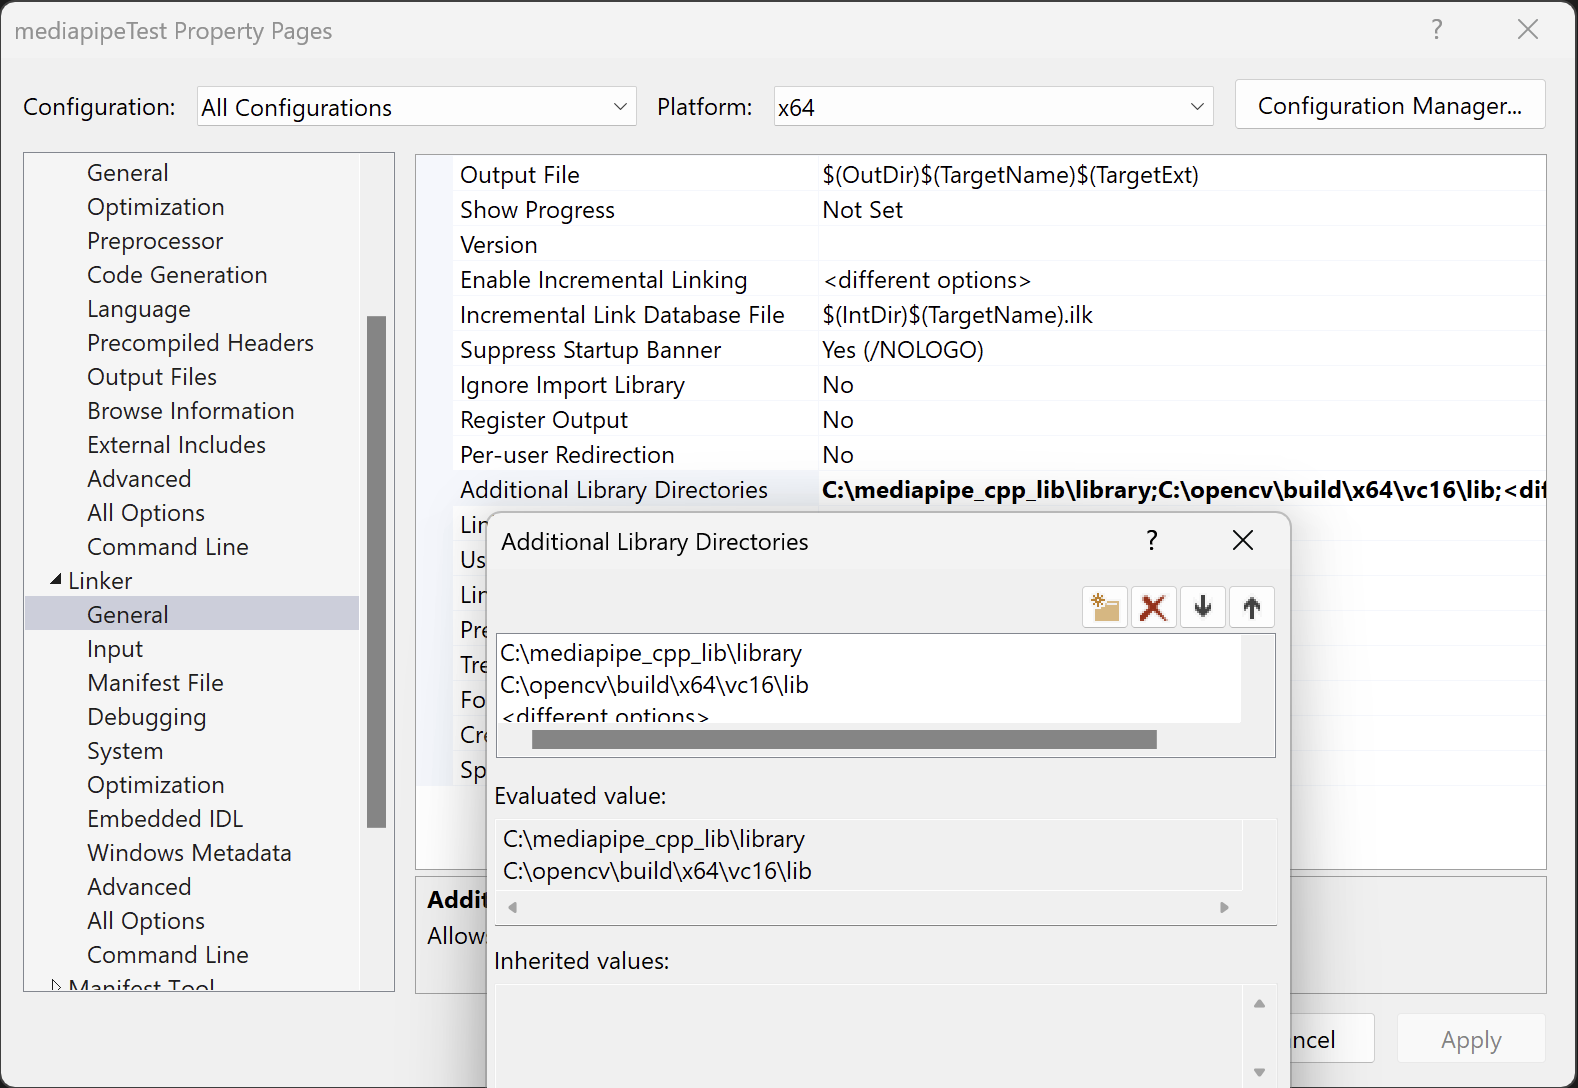
\includegraphics[width=0.7\linewidth]{images-classes/settings2.png}
                \end{minipage}
                \hfill 
                \begin{minipage}[h]{0.49\linewidth}
                    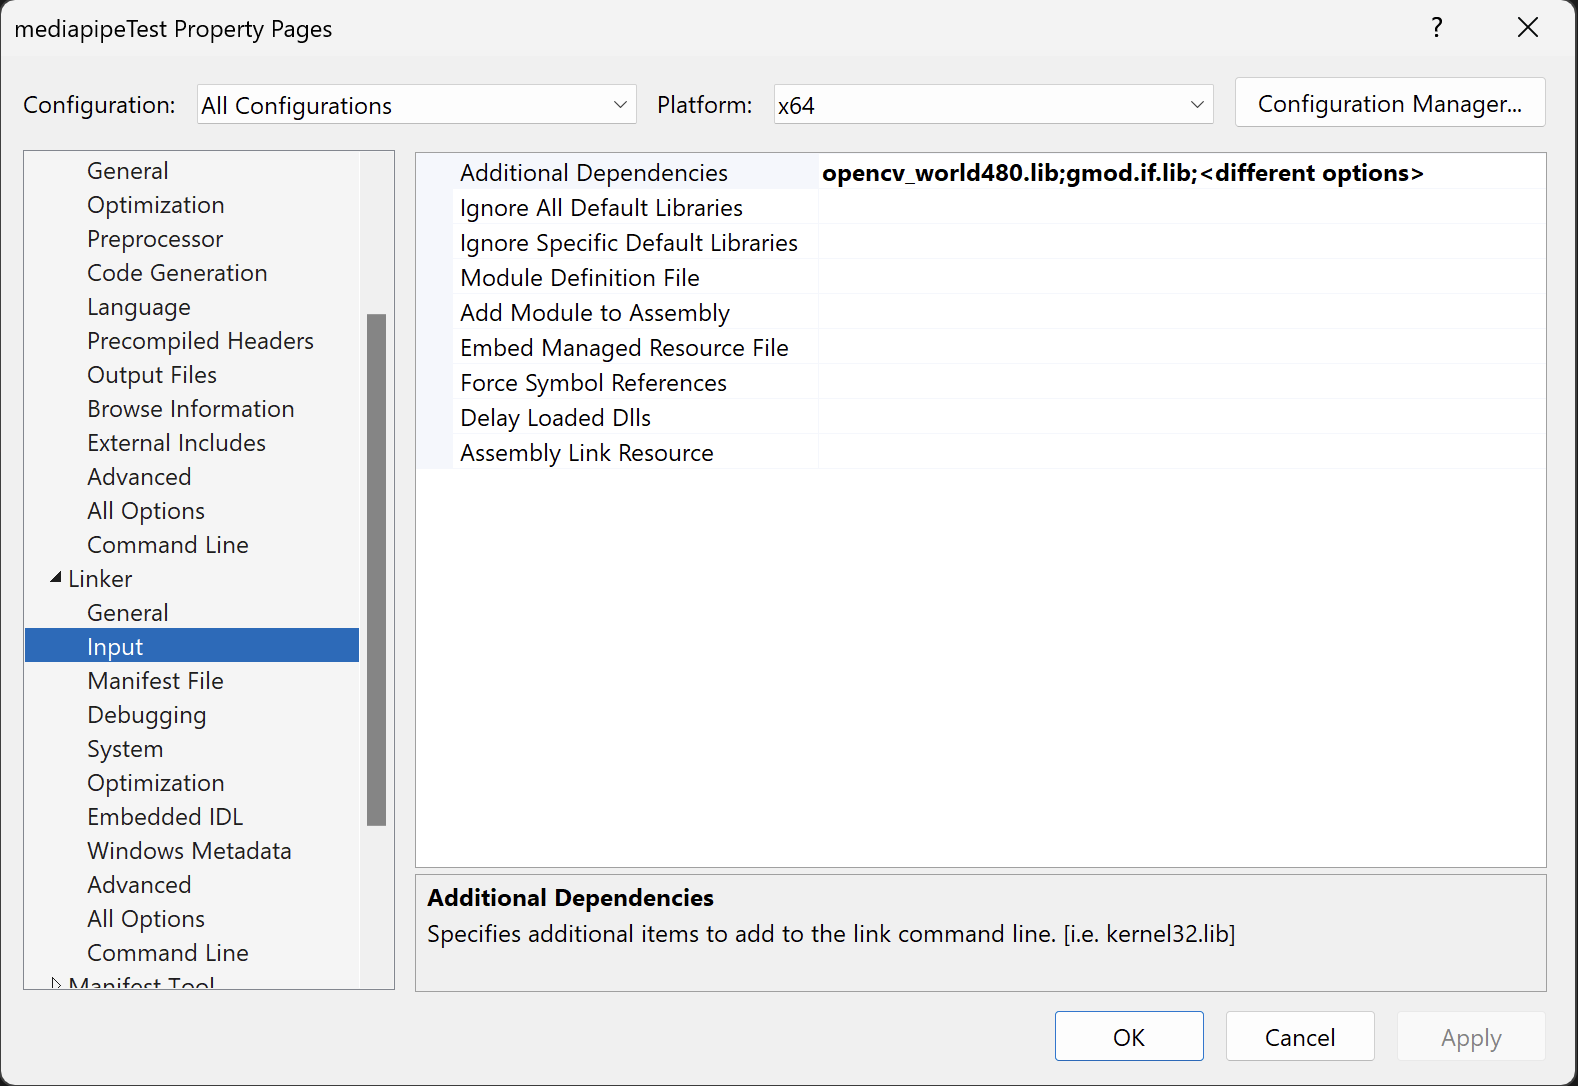
\includegraphics[width=0.7\linewidth]{images-classes/settings3.png}
                \end{minipage}
            \end{center}
            \caption{Настройки Linker}
            \label{ris:settings1}
        \end{figure}
        \begin{figure}[H]
            \center{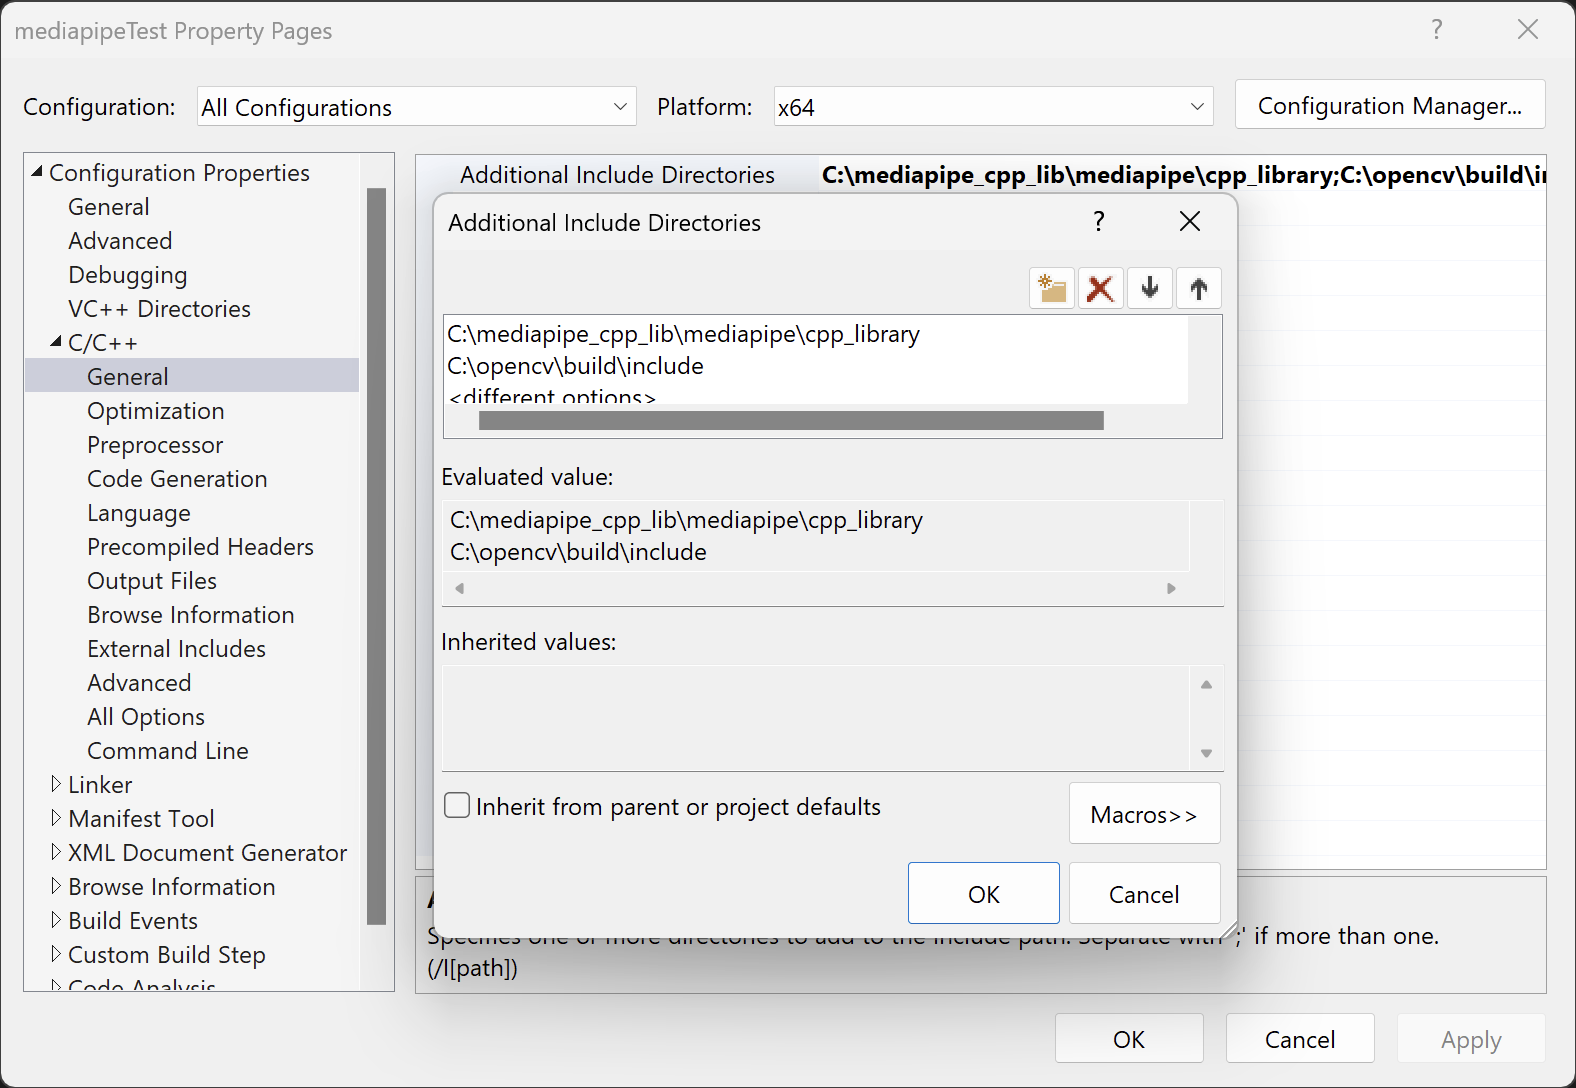
\includegraphics[width=0.6\linewidth]{images-classes/settings1.png}}
            \caption{Настройки C/C++ -> General}
            \label{ris:settings2}
        \end{figure}

        Все готово для запуска тестовой программы:
        \lstinputlisting[language=c++, caption={Основная программа в Visual Studio}]{codeClasses/main.cpp}

        Результат работы программы:
        \begin{figure}[h]
            \begin{center}
                \begin{minipage}[h]{0.49\linewidth}
                    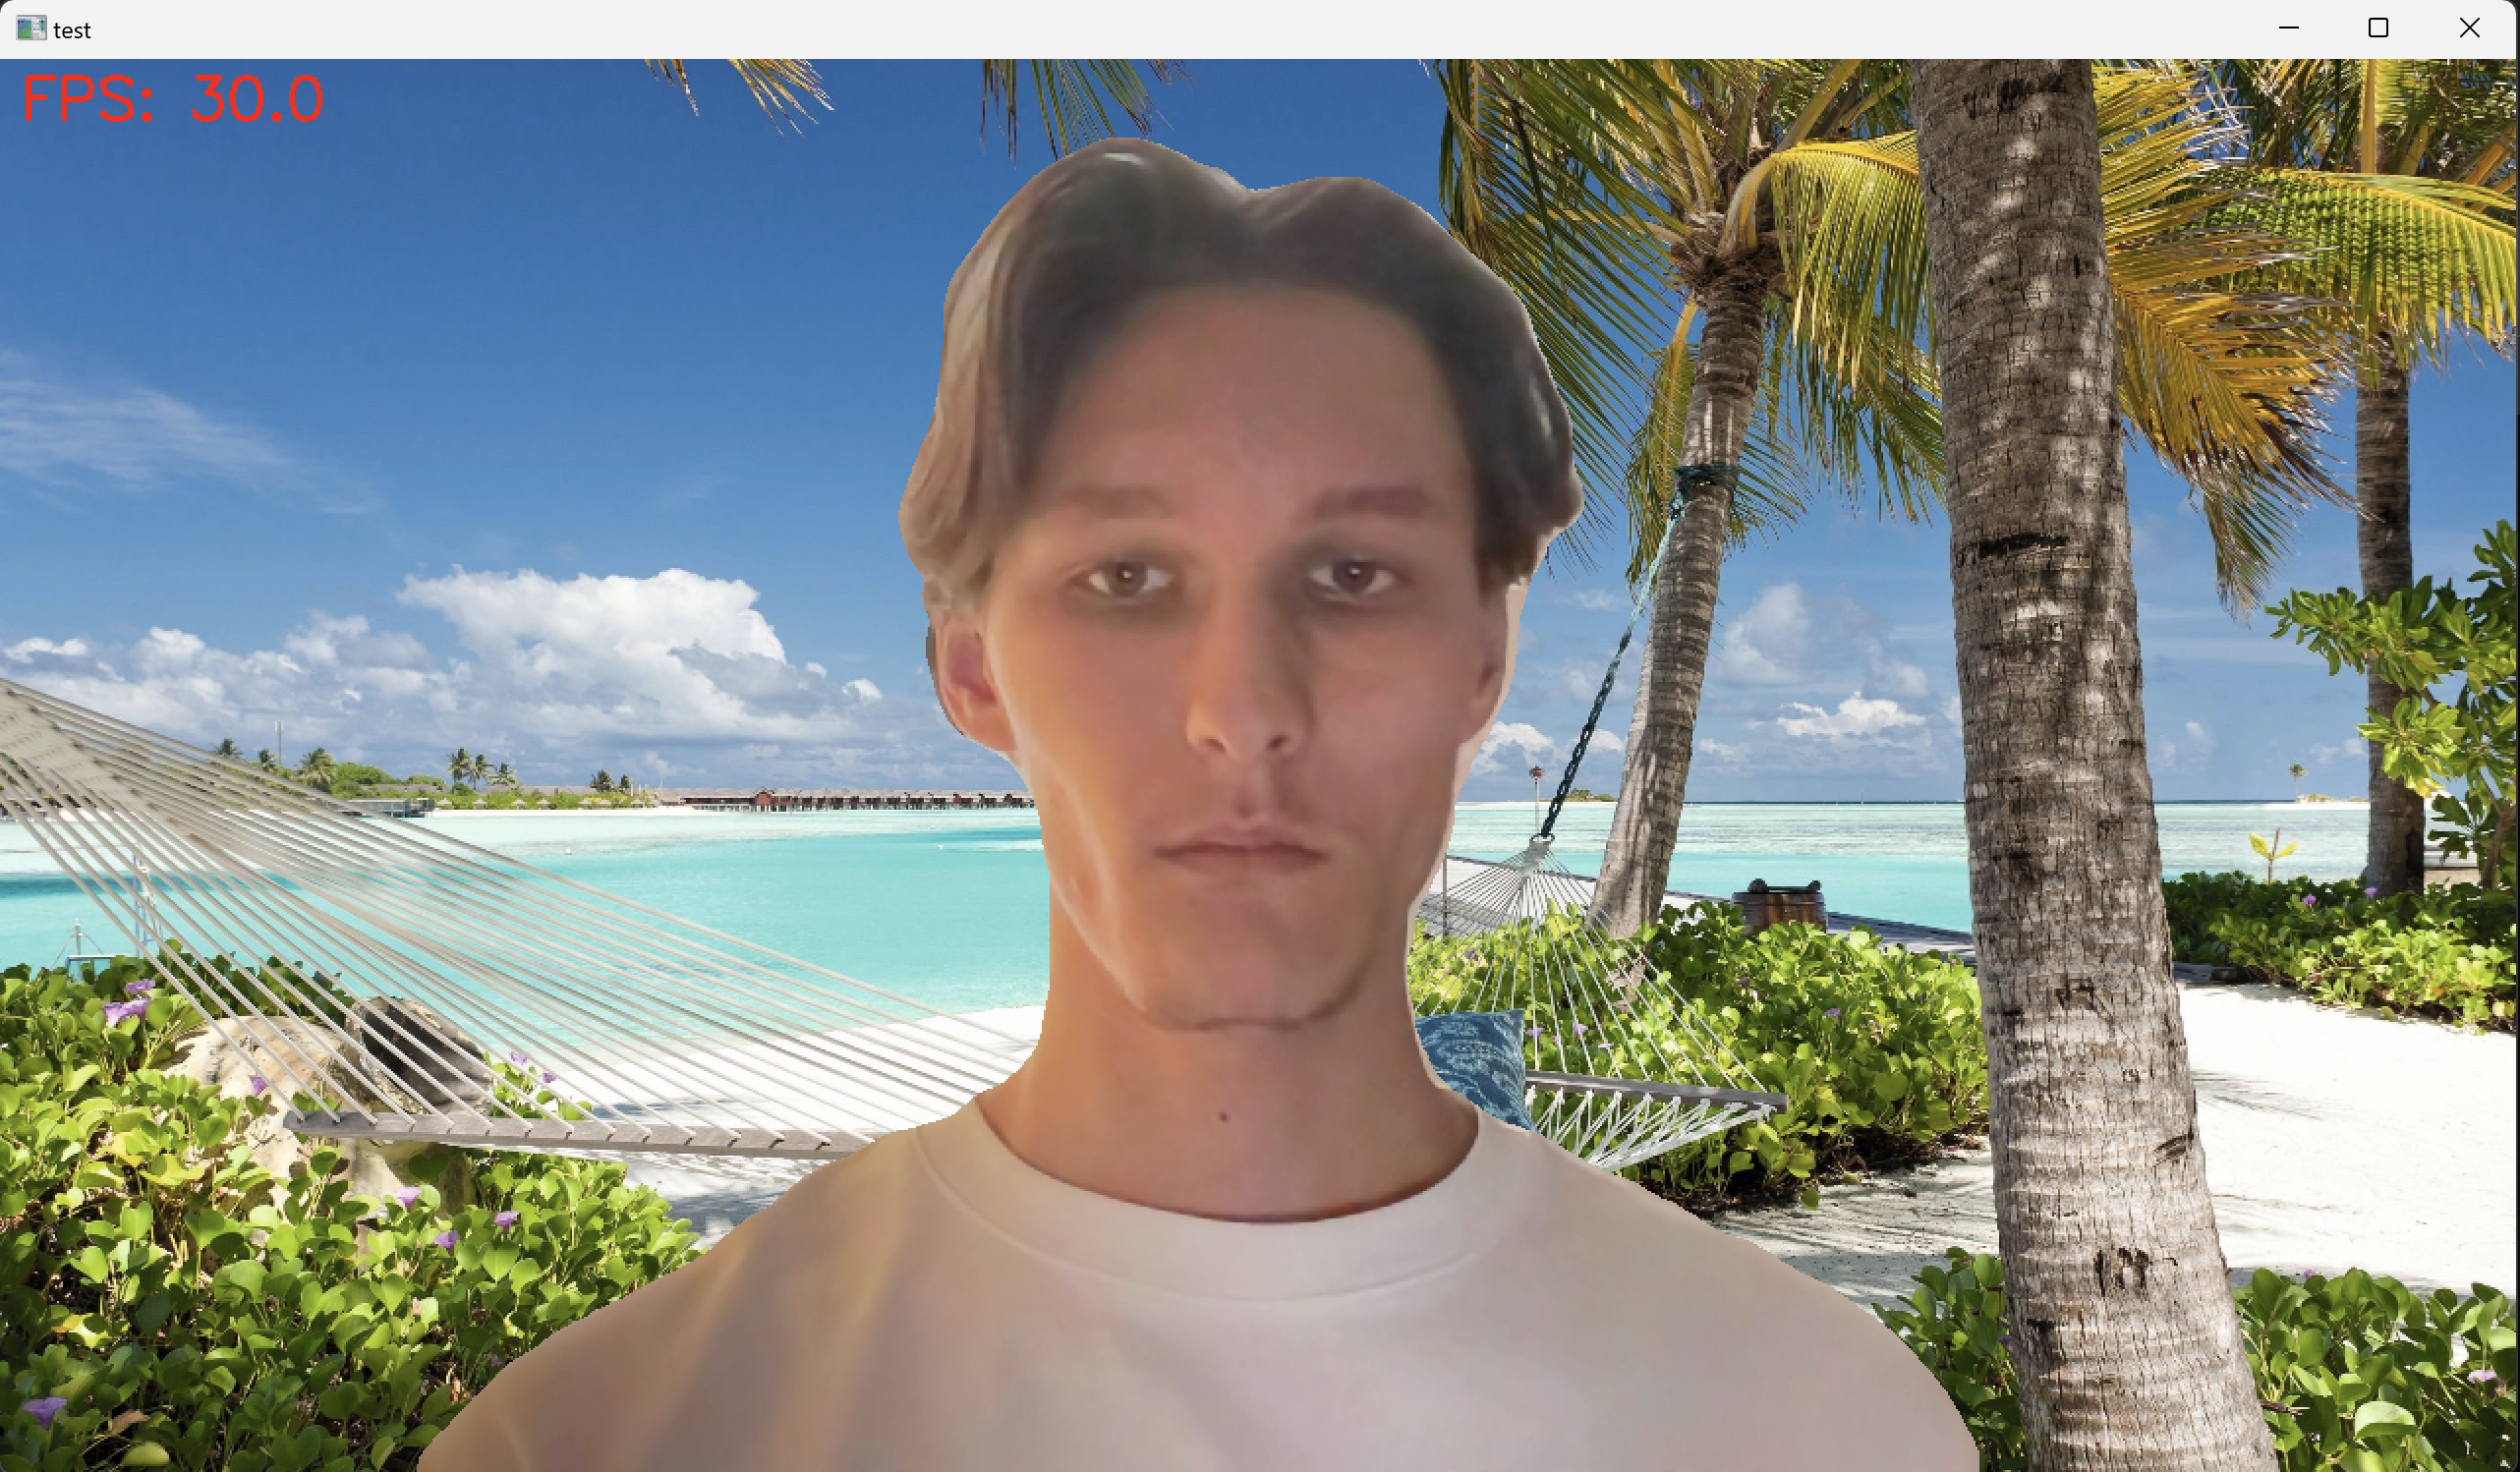
\includegraphics[width=0.7\linewidth]{images-classes/test.png}
                \end{minipage}
                \hfill 
                \begin{minipage}[h]{0.49\linewidth}
                    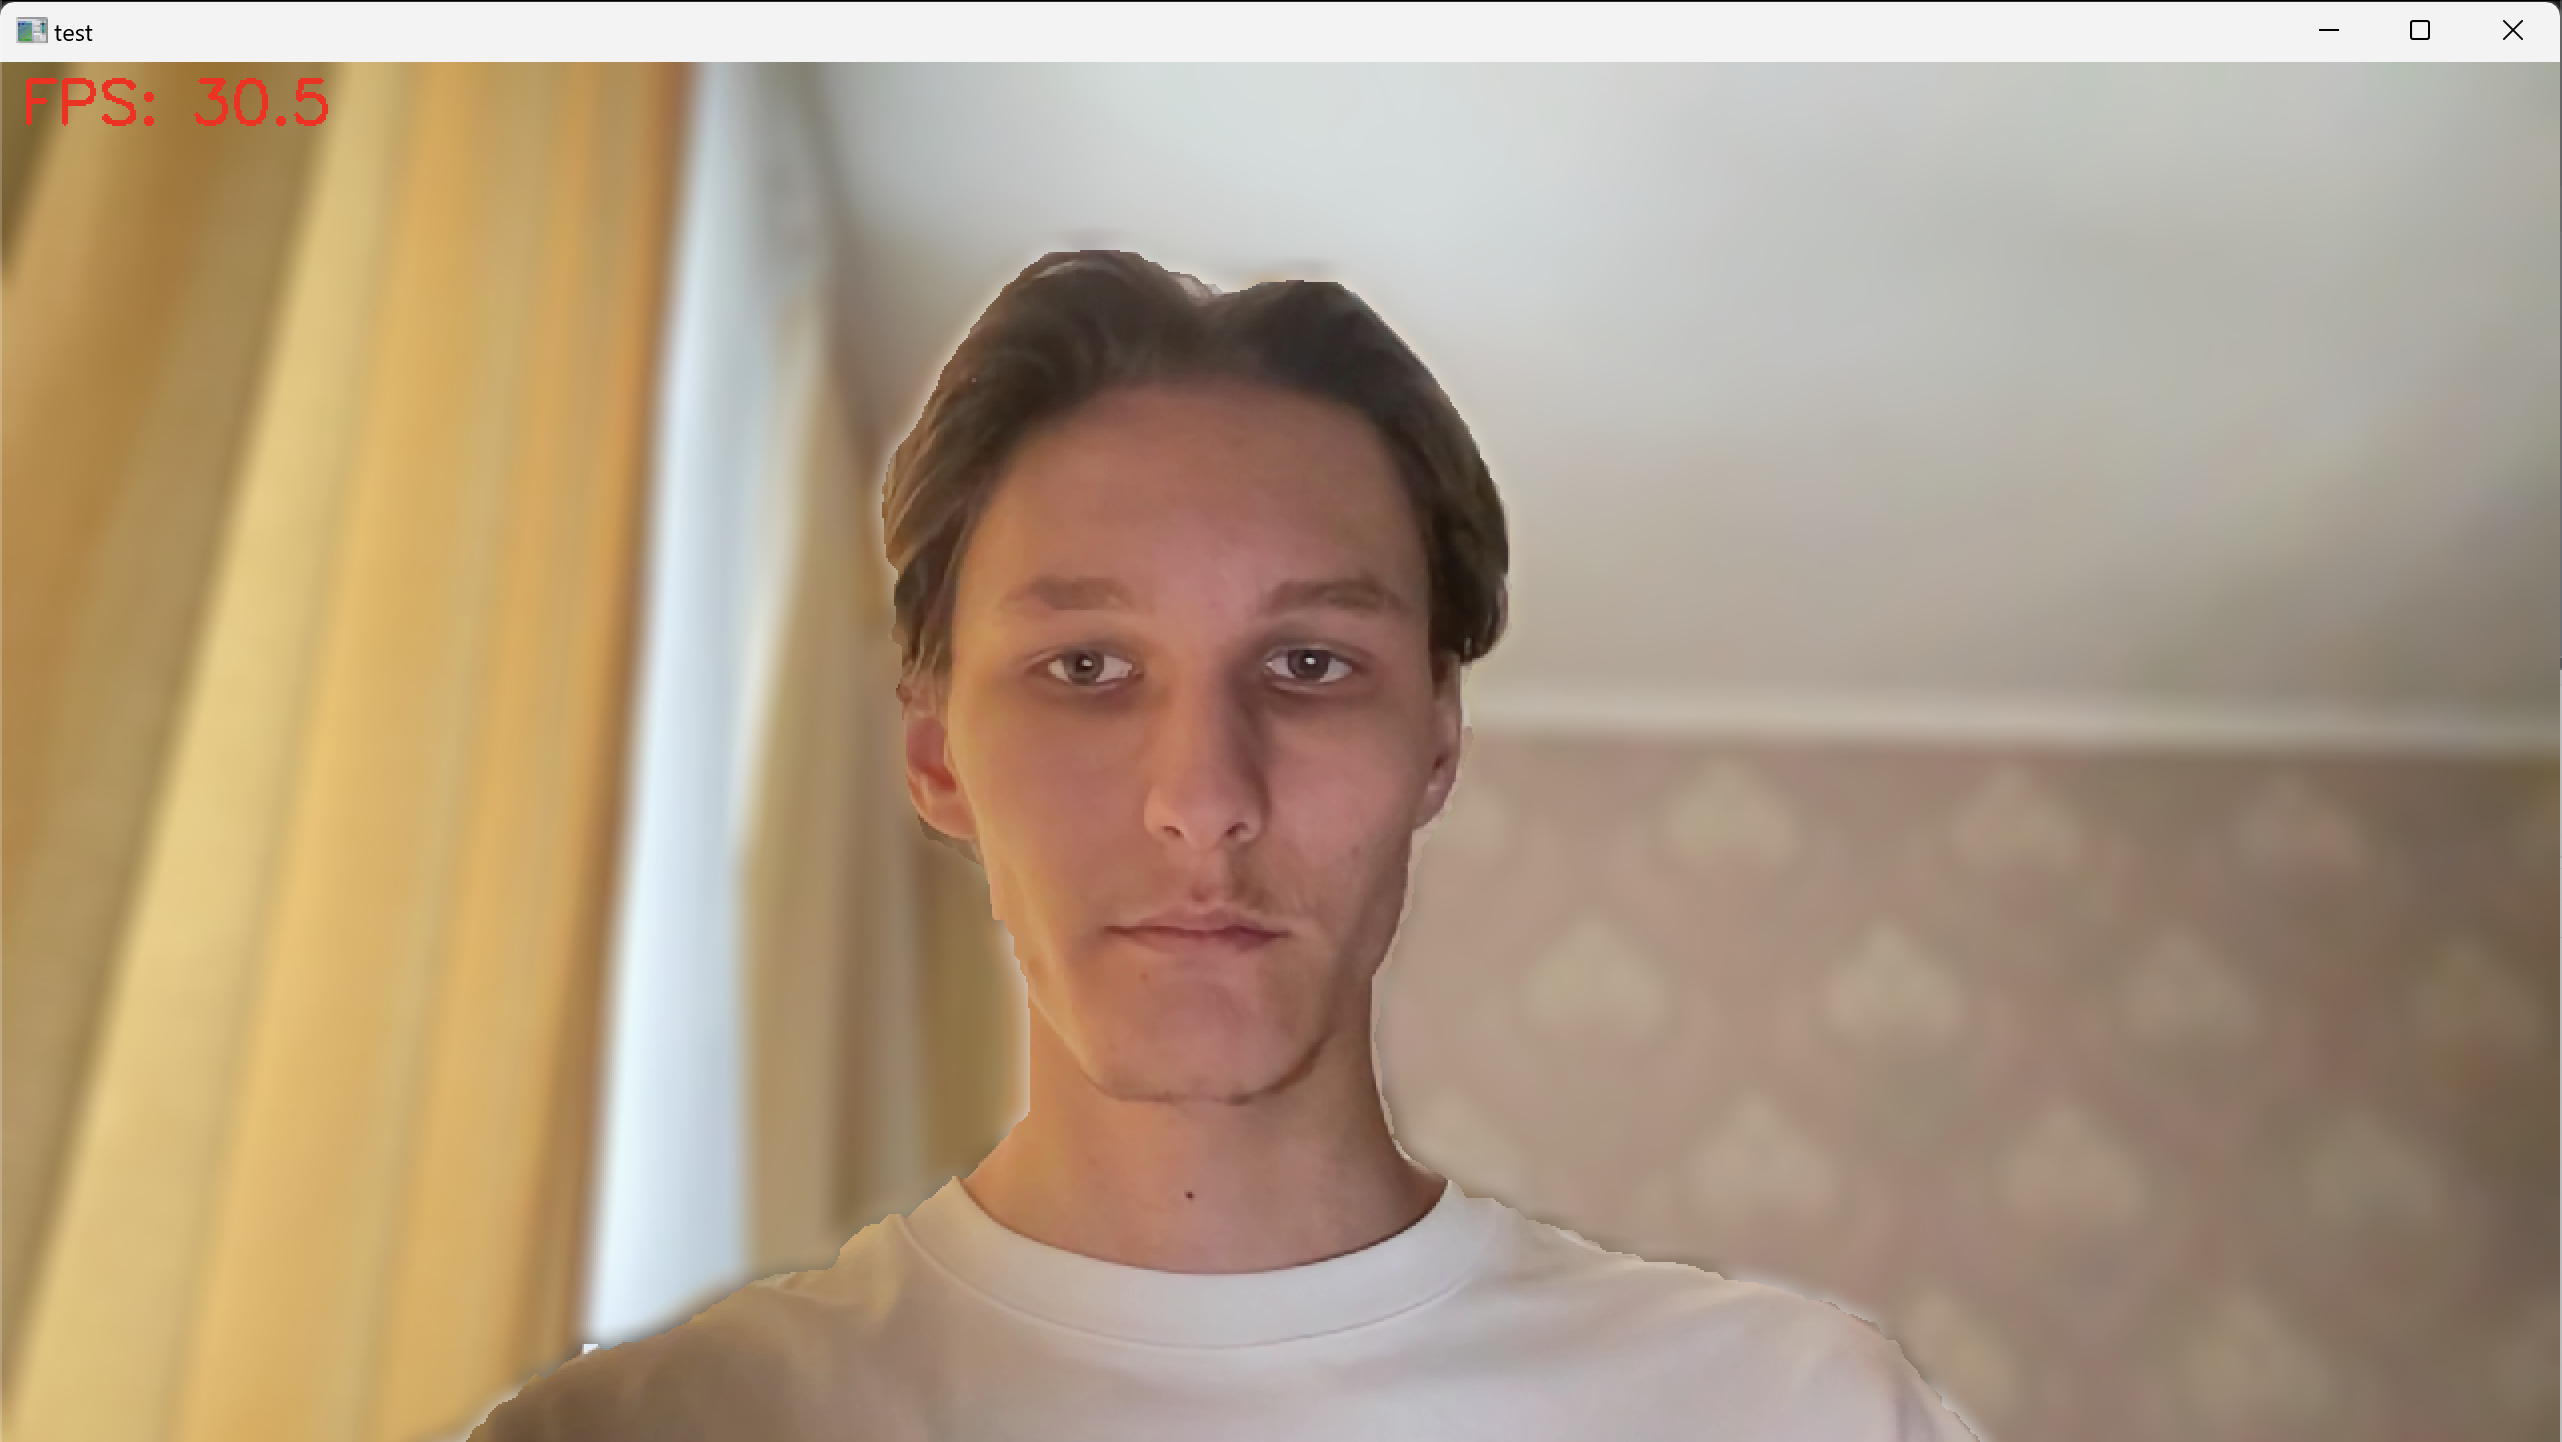
\includegraphics[width=0.7\linewidth]{images-classes/test2.png}
                \end{minipage}
            \end{center}
            \caption{Результат работы программы}
            \label{ris:test}
        \end{figure}
        
    \chapter*{Заключение}
    \addcontentsline{toc}{chapter}{Заключение}
    В ходе проекта:
    \begin{enumerate}
        \item Была рассмотрена задача обработки видеопотока с помощью фреймворка MediaPipe, а также ее применение на прикладном уровне;
        \item Сделан краткий обзор фреймворка MediaPipe;
        \item Выполнен обзор основных элементов конвейера фреймворка MediaPipe;
        \item Резработана архитектура ковейера и реализованы необходимые калькуляторы для него;
        \item Реализованы классы для работы с фреймфорком MediaPipe в среде разработки Visual Studio;
        \item Успешно протестированы результаты работы.
    \end{enumerate}

    \chapter*{Список использованных источников}
    \addcontentsline{toc}{chapter}{Список использованных источников}
    \begin{enumerate}
        \item Google. (2023). MediaPipe Framework [Electronic resource]: Google for Developers. Режим доступа: \href{https://developers.google.com/mediapipe/framework}{https://developers.google.com/mediapipe/framework}. Дата доступа: 12.12.2023
        \item TensorFlow. (2023). Segmentation [Electronic resource]: TensorFlow Lite. Режим доступа: \href{https://www.tensorflow.org/lite/examples/segmentation/overview}{https://www.tensorflow.org/lite/examples/segmentation/overview}. Дата доступа: 12.12.2023
        \item Lugaresi, C., Tang, J., Nash, H., McClanahan, C., Uboweja, E., Hays, M., Zhang, F., Chang, C., Yong, M. G., Lee, J., Chang, W. T., Hua, W., Georg, M., & Grundmann, M. (2019). MediaPipe: A Framework for Building Perception Pipelines [Electronic resource]. Режим доступа: \href{https://arxiv.org/pdf/1906.08172.pdf}{https://arxiv.org/pdf/1906.08172.pdf}. Дата доступа: 12.12.2023
        \item bazel.build. Bazel [Electronic resource]. Режим доступа: \href{https://bazel.build}{https://bazel.build}. Дата доступа: 12.12.2023
    \end{enumerate}
    
\end{document}
